\documentclass[a4papper]{article}

\usepackage[final]{pdfpages}
\usepackage{graphicx}
\usepackage{amssymb, amsmath, amsthm, mathrsfs}
\usepackage{indentfirst}
\usepackage{amsmath}
\usepackage{listings}
\newtheoremstyle{neosn}{0.5\topsep}{0.5\topsep}{\rm}{}{\sc}{.}{ }{\thmname{#1}\thmnumber{ #2}\thmnote{ {\mdseries#3}}}
\theoremstyle{neosn}
\newtheorem{problem}{Problem}

\begin{document}
    \begin{center}
    {\bf Homework 2} \\
        \today \\
        TangLin
    \end{center}

    \problem{Prove that the function $x,y \mapsto \lfloor x^{1/y} \rfloor$ (for positive numbers)
    belongs to the class FP.} \\

    Solution:\\

    I will prove it by constructing Random Access Machine program which can find result in polynomial time,
    and according to the theorem of translation from RAM to MT, the complexity remains polynomial if
    the problems can be solved by RAM in polynomial time. \\

    Then I give the algorithm. \\

    \begin{lstlisting}[label={lst:lstlisting22}]
        // Initialize all the registors we will use.
        a <- 2;
        min_a <- 1;
        max_a <- 2;
        s <- 1;
        tmp <- 1
        t <- 0
        s <- 0

        x <- input_x;
        y <- input_y;

        // Use dichotomy to find suitable results.
        while true:
            t <- input_x;
            s <- 1;
            tmp <- a;

            // Fast exponentiation using dichotomy.
            while t != 0:
                if t % 2 == 0 then {tmp <- tmp*tmp; t <- t/2}
                else {s <- s*tmp; t <- t-1}

        if s > x then {
            tmp <- min_a;
            tmp <- tmp + max_a;
            tmp <- tmp/2;
            a <- tmp;
            max_a <- a;

            if a == min_a then print a;
        }
        else {
            if s == x then {print a;}
            else {
                min_a <- a;
                a <- 2*a;
                max_a <- a;
            }
        }
    \end{lstlisting}

    Let $n = \log{\max{(x,y)}}$, where $x$ and $y$ are positive integer numbers.
    In this algorithm, I need 9 registers to store binary data, and let all the registers
    have the same bits $n$, so $l = O(n)$ and $S = O(1)$. \\
    Now we need to analyze the time complexity.
    In the main while loop, there is another while loop for calculating register $a$ of
    power register $y$.
    Becase I need compare $a^y$ with $b$, and find the final answer.
    Let the time complexity of this loop be $w_2$, we have
    \[
        \begin{array}{l}
            w_2 \leqslant 2(\log(y) + 1) \\
            w_2 = O(n)
        \end{array}
    \]
    In main while loop, I use a dichotomy to find number $a$, the largest number whose $y$-th power
    dose not exceed $x$.
    Let the time complexity of main while loop be $w_1$,so
    \[
        \begin{array}{l}
            w_1 \leqslant 2(\log(x) + 1) \cdot w_2 \cdot (3+6) + 1 \\
            w_1 = O(\log (\max{(x,y)}) \cdot w_2) = O(n)\cdot O(n) = O(n^2)
        \end{array}

    \]

    So $t = O(n^2)$.
    And this algorithm can be executed by RAM in $O(n^2)$ time, and according to the
    theorem we can obtain the time complexity on TM with the same algorithm,
    \[
        t' = O(tSl^2+n) = O(n^2\cdot 1 \cdot n^2+n) = O(n^4) \in \text{FP}.
    \]
    So, we can find the required number in polynomial time by Turing Machine.
    And this problem belongs to the class FP\@. \\


    \problem{Function EVAL which receives
    propositional formula with logical connectors $\land, \lor
    ,\neg$ and values of variables of this formula as arguments
    gives truth value of the formula on the
    variables, prove that function EVAL belongs to the class FP.} \\
    \\
    Solution: \\

    \\
    The proof for this problem is similar to the first problem.
    I will build an algorithm which can be executed by RAM, and explain that
    it can be half in polynomial time on RAM, and print the right answer. \\

    The algorithm: \\

    \begin{lstlisting}[label={lst:lstlisting2}]
        \\ Initial all the rigestors we will use.

        i <- 0                      // The index of character of expression.
        stack_i = [0,0,...,0]       // Rigisters for i.
        stack_ex = ['', ..., '']    // Rigisters for subexpressions.
        stack_paren = [0,...,0]     // Denotes the number of left parenthesises.
        stack_label = ['', ..., ''] // Denotes the next lable.
        stack_left = [0,...,0]
        stack_right = [0,...,0]
        k_left <- 0              // index of left
        k_right <- 0             // index of right
        j <- 0                      // The stack index.
        tmp <- 0                // The value of expreesion or subexpression
        parent <- 0             // The number of parenthesised.
        tmplabel <- 'loop'

        expr <- input

        label_loop:
            if expr[i] == '(' then { paren <- paren + 1 }
            else if expr[i] == ')' then{ paren <- paren - 1 }
            else {
                if expr[i] == '~' then {
                    if expr[i+1] in {0,1} then {
                        tmp <- not tmp
                        if j != 0 then {
                                // There should write judgement statement,
                                // But for convenience, write like this.
                                tmp_lable <- stack_lable[j]
                                expr <- stack_ex[j]
                                i <- stack_i[j]
                                paren <- stack_paren[j]
                                j <- j-1
                                got tmp_lable
                            }
                    }

                    else {
                        stack_i[j] <- i
                        stack_paren[j] <- parent
                        stack_ex[j] <- expr[i:end] //Worst situation,t=O(n)
                        stack_label[j] <- 'lab_not'
                        j <- j+1
                        goto label_loop
                        lable_not:
                            if tmp == 0 then tmp <- 1
                            else tmp <- 0
                            if j != 0 then {
                                tmp_lable <- stack_lable[j]
                                expr <- stack_ex[j]
                                i <- stack_i[j]
                                paren <- stack_paren[j]
                                j <- j-1
                                got tmp_lable
                            }
                    }
                }

                else if expr[i] == '&' then {
                    if expr[i-1] in {0,1} then {
                        stack_left <- expr[i-1]
                        k_left <- k_left+1
                    }

                    else {
                        stack_i[j] <- i
                        stack_paren[j] <- parent
                        stack_ex[j] <- expr[star:i]
                        stack_label[j] <- 'lab_land'
                        j <- j+1
                        goto label_loop
                        label_land:
                            stack_left[k_left] <- tmp
                            k_left <- k_left+1
                            if j != 0 then {
                                tmp_lable <- stack_lable[j]
                                expr <- stack_ex[j]
                                i <- stack_i[j]
                                paren = stack_paren[j]
                                j <- j-1
                                got tmp_lable
                    }

                    if expr[i+1] in {0,1} then {
                        stack_right <- expr[i+1]
                        k_right <- k_right+1
                    }

                    else {
                        stack_i[j] <- i
                        stack_paren[j] <- parent
                        stack_ex[j] <- expr[i:end]
                        stack_label[j] <- 'lab_rand'
                        j <- j+1
                        goto label_loop
                        label_rand:
                            stack_left[k_right] <- tmp
                            k_right <- k_right+1
                            if j != 0 then {
                                tmp_lable <- stack_lable[j]
                                expr <- stack_ex[j]
                                i <- stack_i[j]
                                paren = stack_paren[j]
                                j <- j-1
                                got tmp_lable
                    }

                    k_left < k_left-1
                    k_right < k_right -1
                    tmp <- stack_left[k_left] and stack[k_right]
                    if j != 0 then {
                        tmp_lable <- stack_lable[j]
                        expr <- stack_ex[j]
                        i <- stack_i[j]
                        paren = stack_paren[j]
                        j <- j-1
                        got tmp_lable
                }

                else if expr[i] == '|' then
                    ...
                    // It is very similar to the previous case.
            }

        print tmp

    \end{lstlisting}

    The main idea I used here is Expression Tree.
    For this purpose, our input must be processed applicable form.
    For example, if our input has form
    \[
        x_1 \land x_2 \land x_3 \lor x_4 \lor x_5 \land x_6 \lor \neg x_7
    \]
    According to the associative rules of logical symbols, we well know it is
    equivalent to
    \[
        (x_1 \land x_2 \land x_3) \lor x_4 \lor (x_5 \land x_6) \lor (\neg x_7)
    \]
    But it is not enough for my algorithm, because I find the outmost logical symbol
    based on the parenthesis.
    So I need add more parenthesis
    \[
        (((x_1 \land x_2) \land x_3) \lor x_4) \lor ((x_5 \land x_6) \lor (\neg x_7))
    \]
    All the three formulas are the same, they have the same expression tree

    \includepdfset{postcommand={\thispagestyle{fancy}}}
    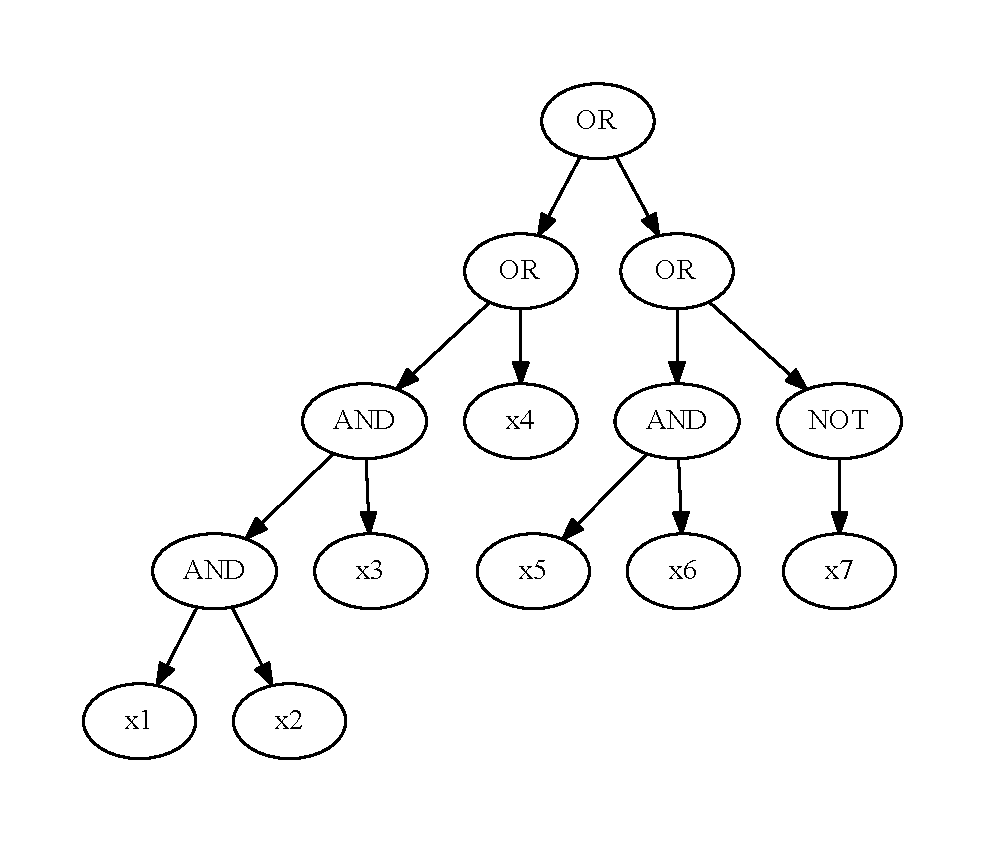
\includepdf{Tree.gv.pdf}

    In my program, it counts the parentheses as number $n_{pa}$, if it meets $($ then let
    increase $n_{pa}$ by $1$, if it meets $)$ then let reduce $n_{pa}$ by 1;
    if it meets a logical symbol and $n_{pa} = 0$ at the same time, then it is the root node
    of expression(subexpression).
    Then evaluate the value of the expression(subexpression). \\
    It is a recursive process, but I translate it to a loop with many stacks which can store
    these statuses. \\

    Now I analyze complexity of this algorithm.
    First, if the input string of expression has $n$ symbols (including parentheses), so we will
    use at most $a\cdot n$ registers, so $S=O(n)$, and every register at most $b \cdot n$ bits, so
    $l=O(n)$, where $a,b$ are some constants.
    And the program evaluates does not exceed $n$ times, because there are less than $n$ logical symbols
    and every logical symbol only need evaluate once.
    So $t=O(n)$. \\

    I have to explain that, in my algorithm I didn't perform actions that receive a formula, and the values
    of arguments of the formula.
    But it is obvious that it can be reached in $O(n)$ time and only use $O(n)$ spaces.
    So the complexity will not change. \\

    Hence, I built an algorithm with $l=O(n), S=O(n), t=O(n)$ by RAM, and according to the theorem, there
    will be a TM with $t=O(tsl^2+n)=O(n^4)$ which can execute this algorithm.
    So this problem belongs to the class FP. \\

    \\ The second solution: \\

    I also consider this problem and try to build a Turing Machine to answer the question.
    I find that is can be achieved in $O(n^3)$ time.
    The main idea is similar to the first one. In this TM $T$, there are some statuses include the most important
    "reset" status, if there are $n$ logical symbols, $T$ will evaluate each logical symbol with values of
    its arguments including removing parentheses in $O(n)$ time, and then reset the head to the initial position
    and reset status to initial status, then there will be at most $n-1$ logical symbols which are not evaluated.
    So,
    \[
        t = O(n \cdot \sum_{i=1}^{n}i ) = O(n^3)
    \]
    It indicates that this problem belongs to the class FP.

\end{document}